%%%%%%%%%%%%%%%%%%%%%%%%%%%%%%%%%%%%%%%%%%%%%%%%%%%%%
%% File: main.tex
%% Author: John Liaperdos (ioannis.liaperdos@gmail.com)
%% Last update: March 31, 2017
%% Description: Provides an example of a PhD Thesis 
%% using the teipel-thesis-en pdfLaTeX class.
%%
%% Character encoding: UTF-8
%%%%%%%%%%%%%%%%%%%%%%%%%%%%%%%%%%%%%%%%%%%%%%%%%%%%%
%
%
%%%%%%
% 1. use the "modern" or "classic" option to switch between 
% a modern or classic font, respectively.
%
% 2. add/remove the "hyperref" option to enable/disable hyperlinks:
% (remember to remove auxiliary files after adding/removing 
% the "hyperref" option).
%
% 3. add/remove the "printer" option to typeset a printer-friendly 
% (grayscale)/color version of the thesis.
%
% 4. use the "watermark" option to indicate a draft copy of the thesis
%
% 5. use the "histinit" option to enable "historiated initials".
% (If used, all chapter initials declared by the \InitialCharacter{}
% macro are enlarged. If ommitted, arguments of \InitialCharacter{}
% are typeset as normal text.)
%
% 6. use the "plain" option to disable tikz graphics in title page
% and part/chapter headers (might help to avoid compilation timeouts).
% Note that "plain" disables CD label and CD cover creation.
%
% 7. use the "noindex" option to (hopefully) avoid compilation timeouts
% when compiling online (disables index generation - note that "\indexGR",
% "\index" invocations need not be removed when toggling this option).
%
% 8. use the "frontispiece" option to typeset a frontispiece at the back of the cover page
%
% 9. use the "letter" option for a US letter page layout, instead of A4
%
% 10. use the "minitoc" option to load and properly initialize the "minitoc" package, 
% that allows typesetting individual tables of contents per chapter.
% (remember to remove auxiliary files after adding/removing 
% the "minitoc" option).
%
%%%%%%%%%%%%%%%%%%%%%%%%%%%%%%%%%%%%%%%%%%%%%%%%%%%%%%%%%%%%%%%%%%%%%%%%%%%%%%%
%
	\documentclass[modern,hyperref,watermark,histinit,frontispiece,minitoc]{teipel-thesis-en}
%
%%%%%%%%%%%%%%%%%%%%%%%%%%%%%%%%%%%%%%%%%%%%%%%%%%%%%%%%%%%%%%%%%%%%%%%%%%%%%%%
%
%
%%%%%%%%%%%%%%%%%%%%%%%%%%%%%%%%%%%%%%%%%%%%%%%%%%%%
%% UNIVERSITY INFO 
%%%%%%%%%%%%%%%%%%%%%%%%%%%%%%%%%%%%%%%%%%%%%%%%%%%%
%
% University Name
%
	\UniversityName{University of Something}
%
% School Name
%
	\SchoolName{The Graduate School}
%
% Department Name
%
	\DepartmentName{Some Department}
%
% Location
%
	\UniversityLocation{Old York}
%
%
%%%%%%%%%%%%%%%%%%%%%%%%%%%%%%%%%%%%%%%%%%%%%%%%%%%%
%% THESIS INFO 
%%%%%%%%%%%%%%%%%%%%%%%%%%%%%%%%%%%%%%%%%%%%%%%%%%%%
%
%% -------------------------------------------------------------------
% Thesis Type
%
	\ThesisType{PhD Thesis}
%
%% -------------------------------------------------------------------
% Thesis Title 
%
% To force line breaks in title, use "\\".
% If different line break locations are to be used for the cover page and the inner title page (page 3) 
% repeat the cover page title as an optional argument of the \title macro, including line breaks.
%
% Examples:
% 1. Automatic title line breaks in cover page and inner title page: 
%	    \title{This is my title}
% 2. Title breaking after ''my'' in both cover page and inner title page:
%	    \title{This is my \\ title}
% 3. Title breaking after ''my'' in cover page, and after ''is'' in inner title page:
%	    \title[This is my \\ title]{This is \\ my title}
%
	\title{My Thesis Title}
%%
%
%% -------------------------------------------------------------------
%% Thesis subtitle (optional)
%
% If no subtitle is required, set argument to blank, or comment-out the \subtitle macro.
%
% Example:
%%	\subtitle{This is my subtitle}
	\subtitle{This is my subtitle}
%
%% -------------------------------------------------------------------
%
%% Author name
%
% For more than one authors, separate with ",".
% Example:
%	\authorName{Albert Einstein, George W. Bush} 
	\authorName{Albert Einstein} 
%
%% -------------------------------------------------------------------
%
%% Supervisor's name
% 
	\supervisor{George Washington}
%
%% -------------------------------------------------------------------
%% Supervisor's title
%
	\supervisorTitle{Professor}
%
%
%% -------------------------------------------------------------------
%% Place and date of publication
%
	\thesisPlaceDate{New York, February 2015}
%
%% -------------------------------------------------------------------
%% Place and date in acknowledgements (if applicable).
%
	\ackPlaceDate{New York, May 2020}
%
%% -------------------------------------------------------------------
%% Approval information
%
	\examinationDate{November 22, 2010}
	\approvalStatement{Approved by ...}
%
%% -------------------------------------------------------------------
%% Copyright Year
%
	\copyrightYear{2030}
%
%% -------------------------------------------------------------------
%% Name of first examiner
%
	\firstExaminer{Professor A}
%
%% -------------------------------------------------------------------
%% Title of first examiner
%
	\firstExaminerTitle{Professor}
%
%% -------------------------------------------------------------------
%% Name of second examiner
%
	\secondExaminer{Professor B}
%
%% -------------------------------------------------------------------
%% Title of second examiner
%
	\secondExaminerTitle{Professor}
%%
%%
%%%%%%%%%%%%%%%%%%%%%%%%%%%%%%%%%%%%%%%%%%%%%%%%%%%%%%%%%%%%%%%%%%%%%%
%% THESIS COLORS: 
%%%%%%%%%%%%%%%%%%%%%%%%%%%%%%%%%%%%%%%%%%%%%%%%%%%%%%%%%%%%%%%%%%%%%%
%%
%% Color for cover and chapters
	\chaptercolor{brown!85!magenta}
%%
%% Color for appendices
	\appendixcolor{brown!60!orange}
%%
%% hyperlink color (ignored if the "hyperref" option is omitted)
    	\hyperlinkcolor{blue}
%%
%% Thesis title foreground color in cover page (ignored if the "plain" option is used)
    	\titlecolor{white}
%%
%% Thesis title background color in cover page (ignored if the "plain" option is used)
    	\titlebackgroundcolor{brown!85!magenta}  
%%
%%
%%%%%%%%%%%%%%%%%%%%%%%%%%%%%%%%%%%%%%%%%%%%%%%%%%%%%%%%%%%%%%%%%%%%%%
%% COVER PAGE IMAGE: 
%%%%%%%%%%%%%%%%%%%%%%%%%%%%%%%%%%%%%%%%%%%%%%%%%%%%%%%%%%%%%%%%%%%%%%
%%
%% Cover page image (optional)
%% If no cover page image is required, set argument to blank, or comment-out the \coverpageimage macro.
%%
%% Syntax:
%%          \coverpageimage{scale factor}{path to cover page image}
%%      or
%%          \coverpageimage[tikz]{scale factor}{TikZ commands}
%%          (commands may include \usetikzlibrary statements, etc.)
%%      
%% Examples:
%%      - Use the image in "figures/rdf.png" scaled by 0.8 (=80%):
%%          \coverpageimage{0.8}{figures/rdf.png}
%%      - Use a TikZ drawing scaled by 0.5 (=50%):
%%          \coverpageimage[tikz]{0.5}{
%%              \draw[thick, magenta] \foreach \x in {18,90,...,306} {
%%                  (\x:4) node{} -- (\x+72:4)
%%                  (\x:4) -- (\x:3) node{}
%%                  (\x:3) -- (\x+15:2) node{}
%%                  (\x:3) -- (\x-15:2) node{}
%%                  (\x+15:2) -- (\x+144-15:2)
%%                  (\x-15:2) -- (\x+144+15:2)
%%              };
%%          }
%%
     \coverpageimage{0.8}{figures/rdf.png}
%%
%%
%%%%%%%%%%%%%%%%%%%%%%%%%%%%%%%%%%%%%%%%%%%%%%%%%%%%%%%%%%%%%%%%%%%%%%
%% MISCELLANEOUS SETTINGS: 
%%%%%%%%%%%%%%%%%%%%%%%%%%%%%%%%%%%%%%%%%%%%%%%%%%%%%%%%%%%%%%%%%%%%%%
%%
% Path to University Logo (all supported formats are allowed)
	\UniversityLogoPath{logo/teikal_logo.eps}
%
% Path to University Logo (grayscale version to be used with the `printer' option)
	\UniversityBWLogoPath{logo/teikal_logo_BW.eps}
%
% Scalefactor for University logos (1 for 100%)
	\LogoScaleFactor{0.9}
% Draft Indication (watermark text to be used with the `watermark' option)
	\draftIndication{--- DRAFT COPY v.2.1. ---}
%
% Frontispiece settings (ignored if the `frontispiece' option is omitted)
%	Syntax: \setFrontispiece[scale factor]{path to frontispiece image}{frontispiece image legend}
	\setFrontispiece[0.8]{figures/aesop.png}{Aesop}
%
%%%%%%%%%%%%%%%%%%%%%%%%%%%%%%%%%%%%%%%%%%%%%%%%%%%%%%%%%%%%%%%%%%%%%%
%
% add custom hyphenation rules here
%\hyphenation{} 
%
%%%%
%
%
%%%%
\begin{document}
%
\maketitle

\beginfrontmatter
	
% Abstract (content in `abstract.tex')
	%%
% 摘要信息
% 本文档中前缀"c-"代表中文版字段, 前缀"e-"代表英文版字段
% 摘要内容应概括地反映出本论文的主要内容,主要说明本论文的研究目的、内容、方法、成果和结论。要突出本论文的创造性成果或新见解,不要与引言相 混淆。语言力求精练、准确,以 300—500 字为宜。
% 在摘要的下方另起一行,注明本文的关键词(3—5 个)。关键词是供检索用的主题词条,应采用能覆盖论文主要内容的通用技术词条(参照相应的技术术语 标准)。按词条的外延层次排列(外延大的排在前面)。摘要与关键词应在同一页。
% modifier: 黄俊杰(huangjj27, 349373001dc@gmail.com)
% update date: 2017-04-15
%%

\cabstract{
摘要内容应概括地反映出本论文的主要内容,主要说明本论文的研究目的、内容、方法、成果和结论。要突出本论文的创造性成果或新见解,不要与引言相混淆。语言力求精练、准确,以300—500字为宜。在摘要的下方另起一行,注明本文的关键词(3—5个)。关键词是供检索用的主题词条,应采用能覆盖论文主要内容的通用技术词条(参照相应的技术术语标准)。按词条的外延层次排列(外延大的排在前面)。摘要与关键词应在同一页。
}
% 中文关键词(每个关键词之间用全角分号“;”分开,最后一个关键词不打标点符号。)
\ckeywords{本科毕业论文;\LaTeX\ 模板;中山大学}

\eabstract{
英文摘要内容与中文摘要相同,以250—400个实词为宜。摘要下方另起一行注明英文关键词(Keywords3—5个)。
}
% 英文文关键词(每个关键词之间用半角分号“;”加空格分开, 最后一个关键词不打标点符号。)
\ekeywords{undergraduate thesis; \LaTeX\ template; Sun Yat-Sen University}


% Dedication
	\thesisDedication{to my parents}
% Acknowledgements (content in `acknowledgements.tex')
	% acknowledgements.tex
%
% Aetf <aetf@unlimitedcodeworks.xyz>
% Copyright 2016 Aetf <aetf@unlimitedcodeworks.xyz>
%
% multiple1902 <multiple1902@gmail.com>
% Copyright 2011~2012, multiple1902 (Weisi Dai)
%
% Project Home: https://github.com/Aetf/xjtuthesis
%
% It is strongly recommended that you read documentations located at
%   https://github.com/Aetf/xjtuthesis/wiki
% in advance of your compilation if you have not read them before.
%
% This work may be distributed and/or modified under the
% conditions of the LaTeX Project Public License, either version 1.3
% of this license or (at your option) any later version.
% The latest version of this license is in
%   http://www.latex-project.org/lppl.txt
% and version 1.3 or later is part of all distributions of LaTeX
% version 2005/12/01 or later.
%
% This work has the LPPL maintenance status `maintained'.
%
% The Current Maintainer of this work is Aetf.
%

\iffalse
感谢国家
\fi

% Table of Contents
	\tableofcontents
% List of Figures
	\listoffigures
% List of Illustrations
	\listofillustrations
% List of Tables
	\listoftables
% List of Algorithms
	\listofalgorithms
% Preface (content in `preface.tex') 
	\begin{preface}
	Preface goes here ...  
\end{preface}
	
\beginmainmatter

%%%%%%%%%%%%%%%%%%%%%%%%%%%%%%%%%%%%%%%%%%%%%%%%%%%%%
%% INCLUDE YOUR CHAPTERS/SECTIONS HERE
%%
% Introduction
	% intro.tex
%
% Aetf <aetf@unlimitedcodeworks.xyz>
% Copyright 2016 Aetf <aetf@unlimitedcodeworks.xyz>
%
% multiple1902 <multiple1902@gmail.com>
% Copyright 2011~2012, multiple1902 (Weisi Dai)
%
% Project Home: https://github.com/Aetf/xjtuthesis
%
% It is strongly recommended that you read documentations located at
%   https://github.com/Aetf/xjtuthesis/wiki
% in advance of your compilation if you have not read them before.
%
% This work may be distributed and/or modified under the
% conditions of the LaTeX Project Public License, either version 1.3
% of this license or (at your option) any later version.
% The latest version of this license is in
%   http://www.latex-project.org/lppl.txt
% and version 1.3 or later is part of all distributions of LaTeX
% version 2005/12/01 or later.
%
% This work has the LPPL maintenance status `maintained'.
%
% The Current Maintainer of this work is Aetf.
%

\chapter{绪论}
\echapter{Preface}

    \section{第一个二级标题}
    \esection{The first section in the Preface}

        \subsection{三级标题}
        \esubsection{Subsection in the Preface}

            \subsubsection{四级标题}
    \section{第二个二级标题}
    \esection{Another section in the Preface}


% Parts/Chapters
	\part{Part A}
	\chapter{Background}
\minitoc
\section{section1}
\subsection{sub-section 1}
\section{section 2}
\InitialCharacter{T}his is another chapter ...

%
\begin{algorithm}[tb]
 	\caption{How to write algorithms}
  	\label{myAlgorithm}
 	\KwData{this text}
 	\KwResult{how to write algorithm with \LaTeX2e }
 	initialization\;
 	\While{not at end of this document}{
  	read current\;
  	\eIf{understand}{
   	go to next section\;
   	current section becomes this one\;
   }{
   go back to the beginning of current section\;
  	}
 	}
\end{algorithm}
%
\newpage
blah blah \vfill ~
%
\begin{algorithm}[tb]
	\caption{An algorithm}
    \uIf{if condition}{
      something if \;
    }
    \uElseIf{elseif condition}{
      something elseif \;
    }
    \Else{
      something else \;
    }
\end{algorithm}
%
    \part{Part B} 
	\chapter{Background}
\minitoc
\section{section 3.1}
\subsection{sub-section 3.1.1}
\section{section 3.2}
\InitialCharacter{T}his is another chapter ...
    \part{Part C}
	\chapter{Background}
\InitialCharacter{T}his is another chapter ...
	\chapter{Background}
\minitoc
\section{section 5.1}
\subsection{sub-section 5.1.1}
\section{section 5.2}
\InitialCharacter{T}his is another chapter ...
% Appendices
	\appendices
	\chapter{Test Appendix}

\section{First Section}
...
	\chapter{Figures}

\begin{verbatim}
\begin{figure}[!ht] 
    \centering
    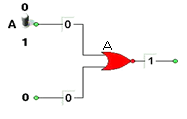
\includegraphics{figures/2.png} 
    \caption{NOR gate.}
    \label{figureB.1}
\end{figure}
\end{verbatim}

\begin{figure}[!ht] 
	\centering
	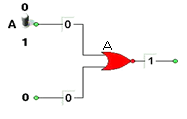
\includegraphics{figures/2.png} 
	\caption{NOR gate.}
	\label{figureB.1}
\end{figure}
	\chapter{Tables}

\begin{verbatim}
\begin{table}[h!]
       \centering
       \caption{My table.}
       \begin{tabular}{|c|c|}
                  \hline
                  \textbf{A} & \textbf{B} \\
                  \hline\hline
                  a11 &  a12 \\
                  \hline
                  a21 &  a22 \\
                  \hline
       \end{tabular}
       \label{table01}
\end{table}
\end{verbatim}

\begin{table}[h!]
	\centering
	\caption{My table.}
	\begin{tabular}{|c|c|}
	    	\hline
	    	\textbf{A} & \textbf{B} \\
	    	\hline\hline
	    	a11 &  a12 \\
	    	\hline
	    	a21 &  a22 \\
	    	\hline
    \end{tabular}
    \label{table01}
\end{table}
	\chapter{Index Generation}


\index{xerox} \index{babel} \index{anna} \index{babylon}

\begin{verbatim}
	\index{xerox} \index{babel} \index{anna} \index{babylon}
\end{verbatim}
	\chapter{Illustrations}
\begin{verbatim}
	\begin{Illustration}[!h] 
	      \centering
	      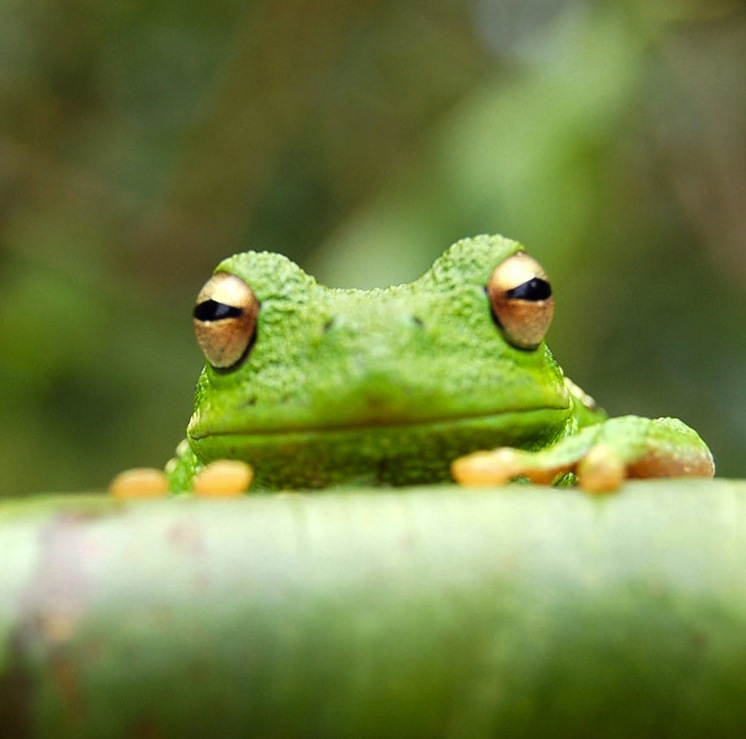
\includegraphics[width=0.5\textwidth]{figures/frog.jpg} 
	      \caption{frog}
	      \label{frog_image}
	\end{Illustration}
\end{verbatim}
\begin{Illustration}[!h] 
	\centering
	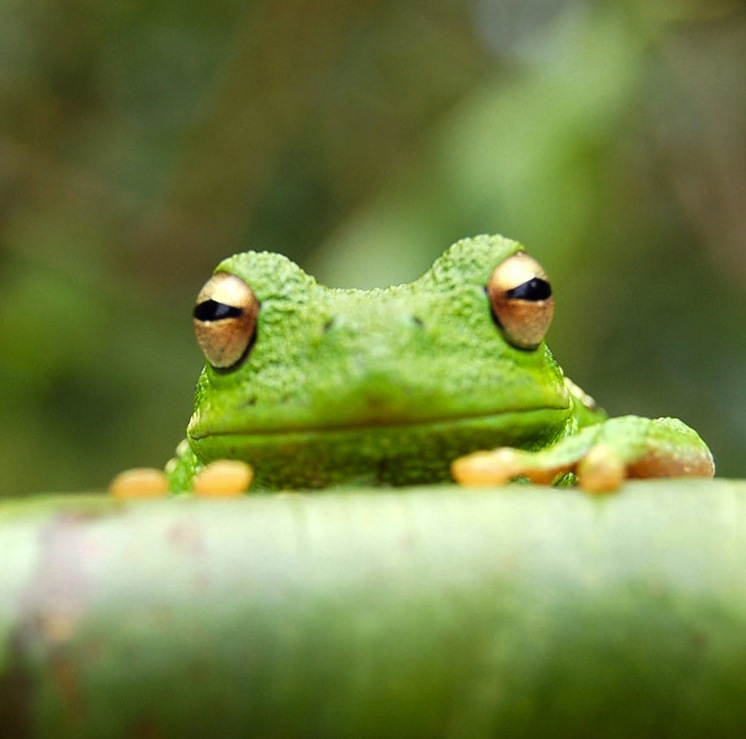
\includegraphics[width=0.5\textwidth]{figures/frog.jpg} 
	\caption{frog}
	\label{frog_image}
\end{Illustration}
	\chapter{Algorithms}
\noindent Algorithms are typeset using the \texttt{algorithm2e} package.
\\[1cm]
Code for floating algorithms:
\begin{verbatim}
  \begin{algorithm}[tb]
      \caption{A floating algorithm}
      \begin{algorithm2e}[H]
        \uIf{if condition}{
            something if \;
            solved \;
        }
        \uElseIf{elseif condition}{
            something elseif \;
        }
        \Else{
            something else \;
        }
     \end{algorithm2e}
  \end{algorithm}
\end{verbatim}

\begin{algorithm}[tb]
	\caption{A floating algorithm}
    \begin{algorithm2e}[H]
      \uIf{if condition}{
          something if \;
          solved \;
      }
      \uElseIf{elseif condition}{
          something elseif \;
      }
      \Else{
          something else \;
      }
  \end{algorithm2e}
\end{algorithm}
  
  \newpage
  
  \noindent For inline algorithms use the "H" option for both \texttt{algorithm} and \texttt{algorithm2e} environments:
\begin{verbatim}
  \begin{algorithm}[H]
      \caption{An "inline" algorithm}
      \begin{algorithm2e}[H]
        \uIf{if condition}{
            something if \;
            solved \;
        }
        \uElseIf{elseif condition}{
            something elseif \;
        }
        \Else{
            something else \;
        }
     \end{algorithm2e}
  \end{algorithm}
\end{verbatim}

  \begin{algorithm}[H]
      \caption{An "inline" algorithm}
      \begin{algorithm2e}[H]
        \uIf{if condition}{
            something if \;
            solved \;
        }
        \uElseIf{elseif condition}{
            something elseif \;
        }
        \Else{
            something else \;
        }
    \end{algorithm2e}
  \end{algorithm}
  
  (and the paragraph continues here ...)
  
  \newpage
  \noindent Of course one might prefer a plain inline presentation:
  \begin{verbatim}
    \begin{algorithm2e}[H]
        \uIf{if condition}{
            something if \;
            solved \;
        }
        \uElseIf{elseif condition}{
            something elseif \;
        }
        \Else{
            something else \;
        }
    \end{algorithm2e}
\end{verbatim}

Text starts here ...

     \begin{algorithm2e}[H]
        \uIf{if condition}{
            something if \;
            solved \;
        }
        \uElseIf{elseif condition}{
            something elseif \;
        }
        \Else{
            something else \;
        }
    \end{algorithm2e}

... and continues here.    
% Bibliography/References (BiBTeX items in `references.bib')
	\bibliography{IEEEabrv,references}
% Abbreviations (content in `abbreviations.tex') 
	\includeabbreviations{abbreviations}
% Glossary (content in `glossary.tex') 
	\includeglossary{glossary}
%%%%%%%%%%%%%%%%%%%%%%%%%%%%%%%%%%%%%%%%%%%%%%%%%%%%
% Index
	\printindices
%
%%%%%%%%%%%%%%%%%%
%%%%%%%%%%%%%%%%%%

%% Create CD labels:

	\definecdlabeloffsets{0}{-0.65}{0}{0.55} % upper label x offset [cm] (default=0) /  upper label y offset [cm] (default=0) /  lower label x offset [cm] (default=0) /  lower  label y offset [cm] (default=0) -- For Q-Connect KF01579 labels use the following offset values: {0}{-0.65}{0}{0.55}

	\createcdlabel{This is my PhD \\ Thesis Title}{My Name}{October}{2014}{8} % thesis title / author name / month / year / title area width in cm (recommended value: 8) 

%%
%% Create CD case covers:

	\createcdcover{This is my PhD \\ Thesis Title}{My Name}{October}{2014}{10} % thesis title / author name / month / year / title area width in cm (recommended value: 10) 

%%
%
\end{document}

%%%%%%%%%%%%%%%%%%%%%%%%%%%%%%%%%%%%%%%%%%%%%%%%%%%%